\subsection{Pengujian Pemetaan Ruangan pada Robot di Simulasi}
\label{subsec:slamsimulasi}

Pengujian pemetaan ruangan di simulasi dilakukan dengan cara menjalankan ruangan \emph{indoor} pada simulator Gazebo dan menjalankan \emph{RTAB-Map node} yang melakukan pemetaan ruangan dari data yang dikirimkan model robot yang ada di simulasi.
Seperti yang dapat dilihat pada gambar \ref{fig:rosgraphslamsimulation},
  \emph{node} \lstinline{/depth_camera_plugin} akan mengirimkan data \emph{depth camera} melalui tiga buah \emph{topic} ke \emph{node} \lstinline{/rtabmap},
  sedangkan \emph{node} \lstinline{/navigation_plugin} akan mengirimkan data melalui \emph{topic} \lstinline{/odom} ke \emph{node} \lstinline{/rtabmap}.

\begin{figure}[ht]
  \centering
  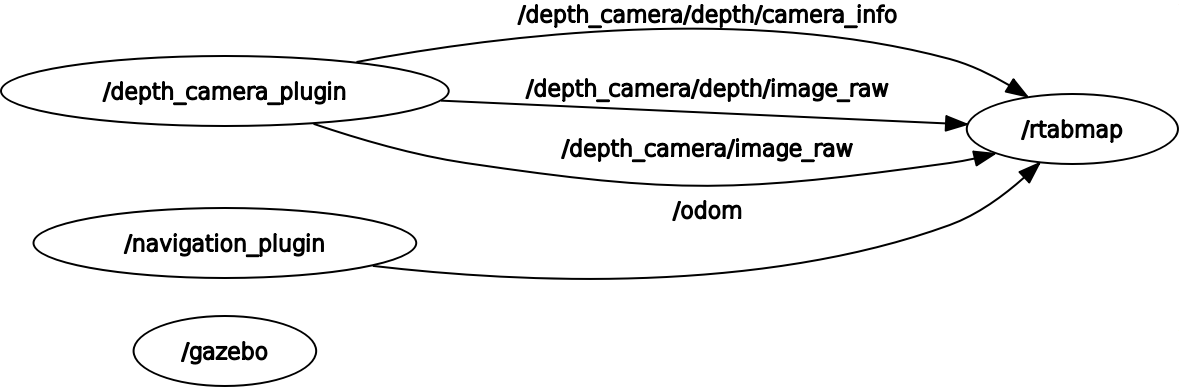
\includegraphics[width=0.95\textwidth,keepaspectratio]{gambar/rosgraph-slam-simulation.png}
  \caption{Relasi antar-\emph{node} dari pengujian pemetaan ruangan pada robot di simulasi.}
  \label{fig:rosgraphslamsimulation}
\end{figure}

\emph{RTAB-Map node} kemudian akan memproses keseluruhan data yang didapat dari komponen \emph{depth camera} dan navigasi untuk melakukan pemetaan pada ruangan yang ada di simulasi.
Seperti yang dapat dilihat pada gambar \ref{fig:hasilpemetaan},
  gambar pertama menunjukkan tangkapan layar yang ada di simulasi ketika robot sedang bergerak sambil melakukan pemetaan ruangan,
  sedangkan gambar kedua menunjukkan tangkapan layar dari hasil pemetaan yang ditampilkan secara visual oleh RTAB-Map.

Dari hasil pemetaan tersebut,
  dapat dilihat bahwa citra berwarna dan citra kedalaman yang diterima diubah kedalam bentuk \emph{point cloud} oleh RTABMap sehingga menghasilkan bentuk peta seperti yang ada di visualisasi tersebut.
Di dalam visualisasi tersebut juga terlihat bentuk lintasan yang telah dilalui robot selama melakukan pemetaan sebagai garis dengan titik berwarna biru.

\begin{figure}[ht]
  \centering
  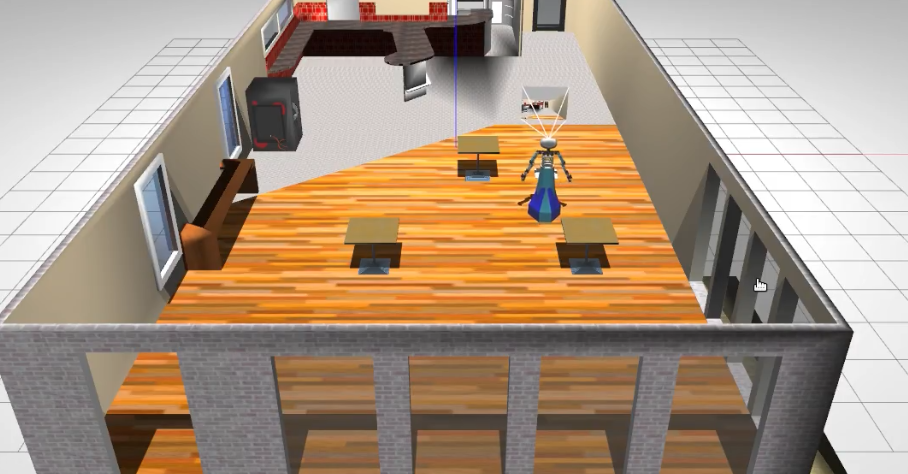
\includegraphics[height=0.26\textwidth,keepaspectratio]{gambar/proses-pemetaan.png}
  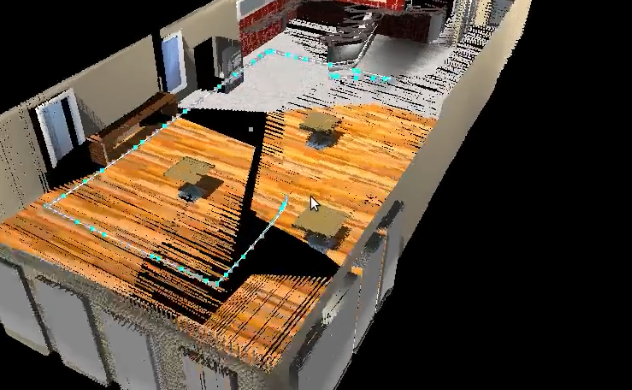
\includegraphics[height=0.26\textwidth,keepaspectratio]{gambar/hasil-pemetaan.png}
  \caption{Proses dan hasil pemetaan ruangan pada robot di simulasi.}
  \label{fig:hasilpemetaan}
\end{figure}
